\documentclass[12pt]{article}
\usepackage[utf8]{inputenc}
\usepackage[usenames]{color}
\usepackage[margin=1in]{geometry} 
\usepackage{amsmath,amsthm,amssymb,graphicx,mathtools,tikz,hyperref, pgfplots, listings, pdfpages}
\usetikzlibrary{positioning}
\newcommand{\n}{\mathbb{N}}
\newcommand{\z}{\mathbb{Z}}
\newcommand{\q}{\mathbb{Q}}
\newcommand{\cx}{\mathbb{C}}
\newcommand{\real}{\mathbb{R}}
\newcommand{\field}{\mathbb{F}}
\newcommand{\ita}[1]{\textit{#1}}
\newcommand{\com}[2]{#1\backslash#2}
\newcommand{\oneton}{\{1,2,3,...,n\}}
\newcommand\idea[1]{\begin{gather*}#1\end{gather*}}
\newcommand\ef{\ita{f} }
\newcommand\eff{\ita{f}}
\newcommand\proofs[1]{\begin{proof}#1\end{proof}}
\newcommand\inv[1]{#1^{-1}}
\newcommand\setb[1]{\{#1\}}
\newcommand\en{\ita{n }}
\newcommand{\vbrack}[1]{\langle #1\rangle}


\newenvironment{theorem}[2][Teorema]{\begin{trivlist}
\item[\hskip \labelsep {\bfseries #1}\hskip \labelsep {\bfseries #2.}]}{\end{trivlist}}
\newenvironment{lemma}[2][Lema]{\begin{trivlist}
\item[\hskip \labelsep {\bfseries #1}\hskip \labelsep {\bfseries #2.}]}{\end{trivlist}}
\newenvironment{exercise}[2][Ejercicio]{\begin{trivlist}
\item[\hskip \labelsep {\bfseries #1}\hskip \labelsep {\bfseries #2.}]}{\end{trivlist}}
\newenvironment{reflection}[2][Reflexión]{\begin{trivlist}
\item[\hskip \labelsep {\bfseries #1}\hskip \labelsep {\bfseries #2.}]}{\end{trivlist}}
\newenvironment{proposition}[2][Proposición]{\begin{trivlist}
\item[\hskip \labelsep {\bfseries #1}\hskip \labelsep {\bfseries #2.}]}{\end{trivlist}}
\newenvironment{corollary}[2][Corolario]{\begin{trivlist}
\item[\hskip \labelsep {\bfseries #1}\hskip \labelsep {\bfseries #2.}]}{\end{trivlist}}
 \hypersetup{
 colorlinks,
 linkcolor=blue
 }

\renewcommand{\ttdefault}{pcr}
\lstdefinestyle{C}{language=C,
    basicstyle=\ttfamily,
    keywordstyle=\bfseries,
    showstringspaces=false,
    morekeywords={include, printf},
	keepspaces=true,numbers=left,xleftmargin=2em,frame=shadowbox,framexleftmargin=0 em, rulesepcolor = \color{black}
}
\lstdefinestyle{linuxterminal}{language=bash,
    basicstyle=\ttfamily,
    keywordstyle=\bfseries,
    showstringspaces=false,
    morekeywords={include, printf},
	keepspaces=true,
	frame=TLRB
}

\begin{document}
	\date{06-02-2018}
	
	
	\title{\textbf{\textcolor{red}{DESIGN REPORT}}}
	\author{Alejandro Santorum Varela - alejandro.santorum@estudiante.uam.es\\David Cabornero Pascual - david.cabornero@estudiante.uam.es\\Autonomous University of Madrid}
	\maketitle
	
\tableofcontents
\newpage


\section{Introduction}
In the next document we are explaining and collecting the different diagrams that are made before the coding and implementation phase in a project.\\\\
We are looking forward to have done it all well and it is clarified nicely.


\section{Class diagram}
The class diagram is attached in another page because of its size.\\There is not too much to explain, we have design the class diagram using PlantUML becuase it places everything efficiently.\\\\ In addiction, we remind you we omitted cardinality equal to one in the arrows, and the methods' arguments might change at the implementation phase, it will be clarified as soon as we learn to code professionally in Java.


\section{State diagrams}
\subsection{Offer state diagram}
Here we are showing the state diagram of the class Offer, that we consider it is the hardest to design:
\begin{center}
	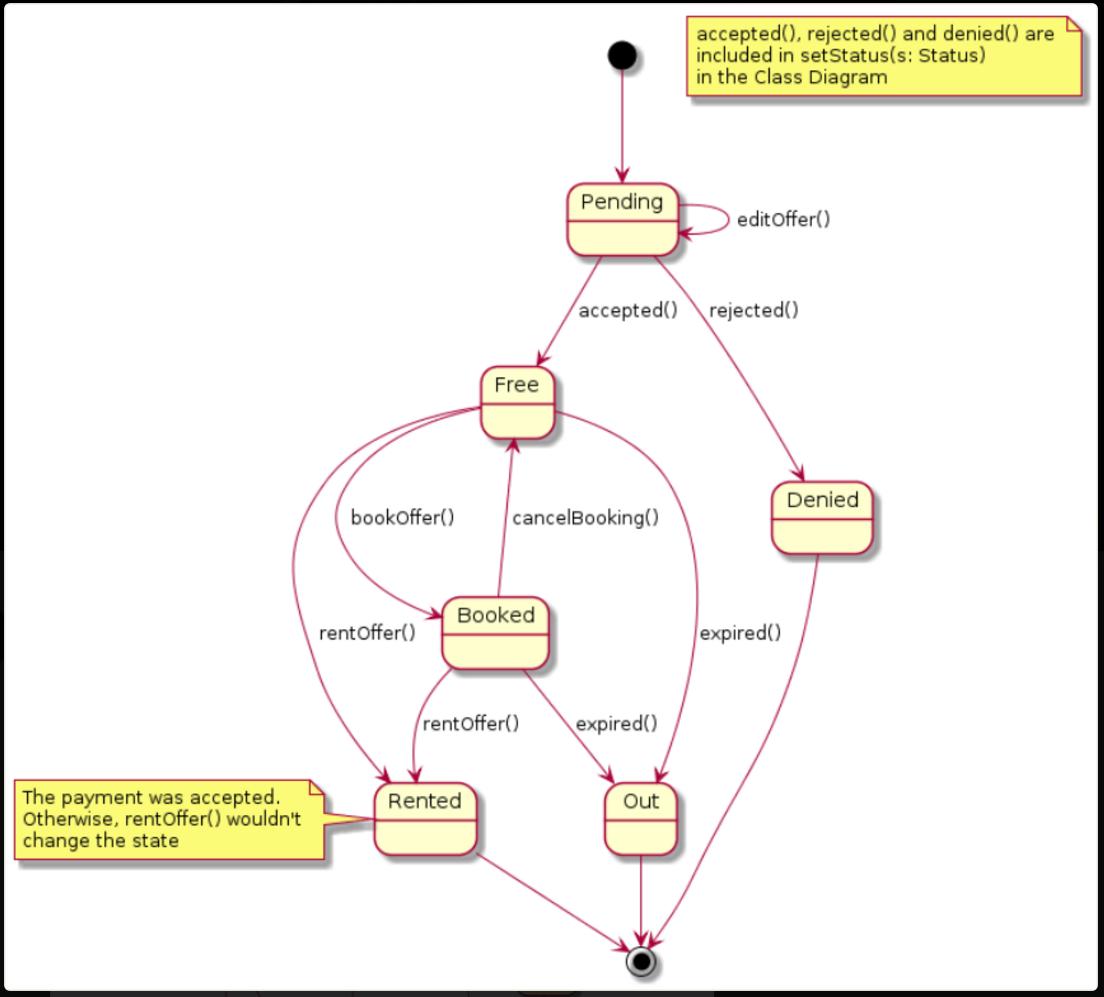
\includegraphics[scale=0.8]{states2.PNG}
\end{center}
Let's comment a little bit this diagram: first, the initial state of an offer is always PENDING state, because every offer has to be approved by the manager before even being available to rent/book.\\\\ 
If the offer is rejected, it is sent to DENIED state that can be considered a final state, that's why its array has no method, we are just indicating DENIED is a final state.\\\\
On the other hand, if it is accepted it is sent to the FREE state, we the offer is declared to be rented.\\In the FREE state, the offer can go to BOOKED state if any user books the offer, or it can go to RENTED state directly, as long as \textbf{the payment is accepted before, otherwise rentOffer() isn't called and it does not change its state}. It has the same behavior in the transiction between BOOKED and RENTED states.\\ It's important to clarify that RENTED state is a final state, that's the reason why there is no methond between RENTED and the final state UML sysbol.\\\\
Finally, OUT state is also considered a final state (same reason as RENTED and DENIED) and an offer reaches this state whenever its deathlines end.\\\\
To clarify, the methods accepted(), rejected() and denied() are different expressions of setStatus(argum: Status), but we have changed its names to make it more intuitive.

\subsection{Renter state diagram}
Here we are showing the state diagram of the class Renter. It is not quite difficult, but our application has not got too much complicated class states.
\begin{center}
	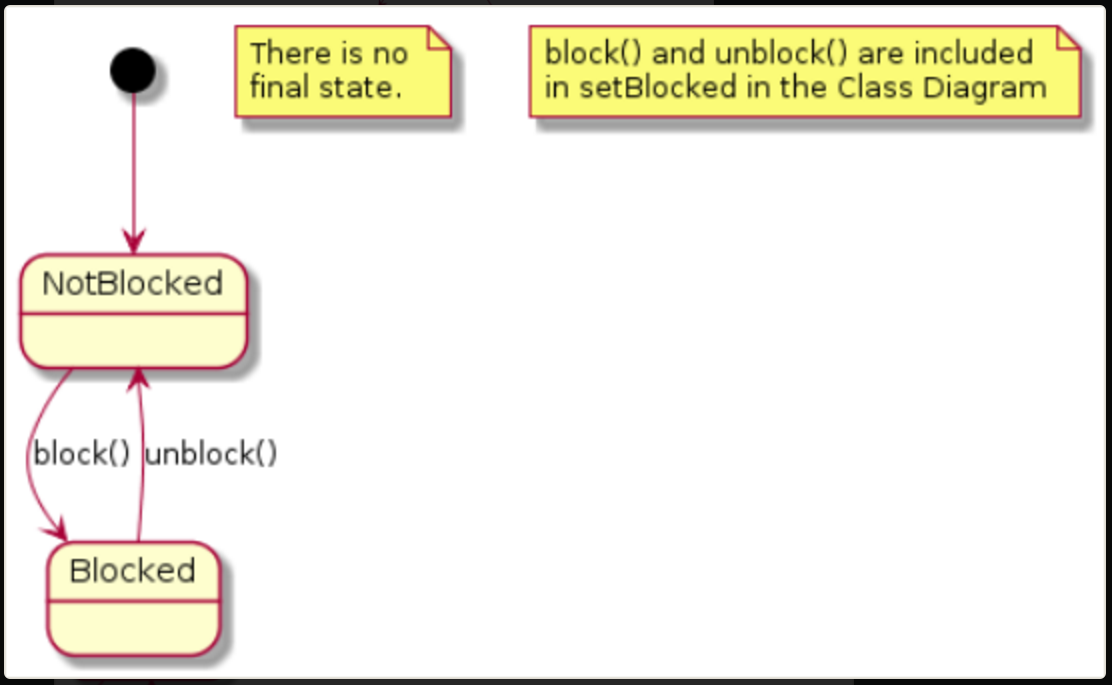
\includegraphics[scale=1]{states1.PNG}
\end{center}
There is no final state in this state diagram because a renter user is either blocked or not blocked, but none of them goes to a final state, they are just swapped depending on its credit card status.\\\\
It's important to remark that block() and unblock() are different names of the same method: setBlocked(), but it is changed in order to clarify it a little bit more.

\section{Sequence diagrams}
\subsection{Make an offer sequence diagram}
Just down below we show the sequence diagram of making an offer. Check out the comments in yellow boxes that appear in the diagram, they can be helpful.
\begin{center}
	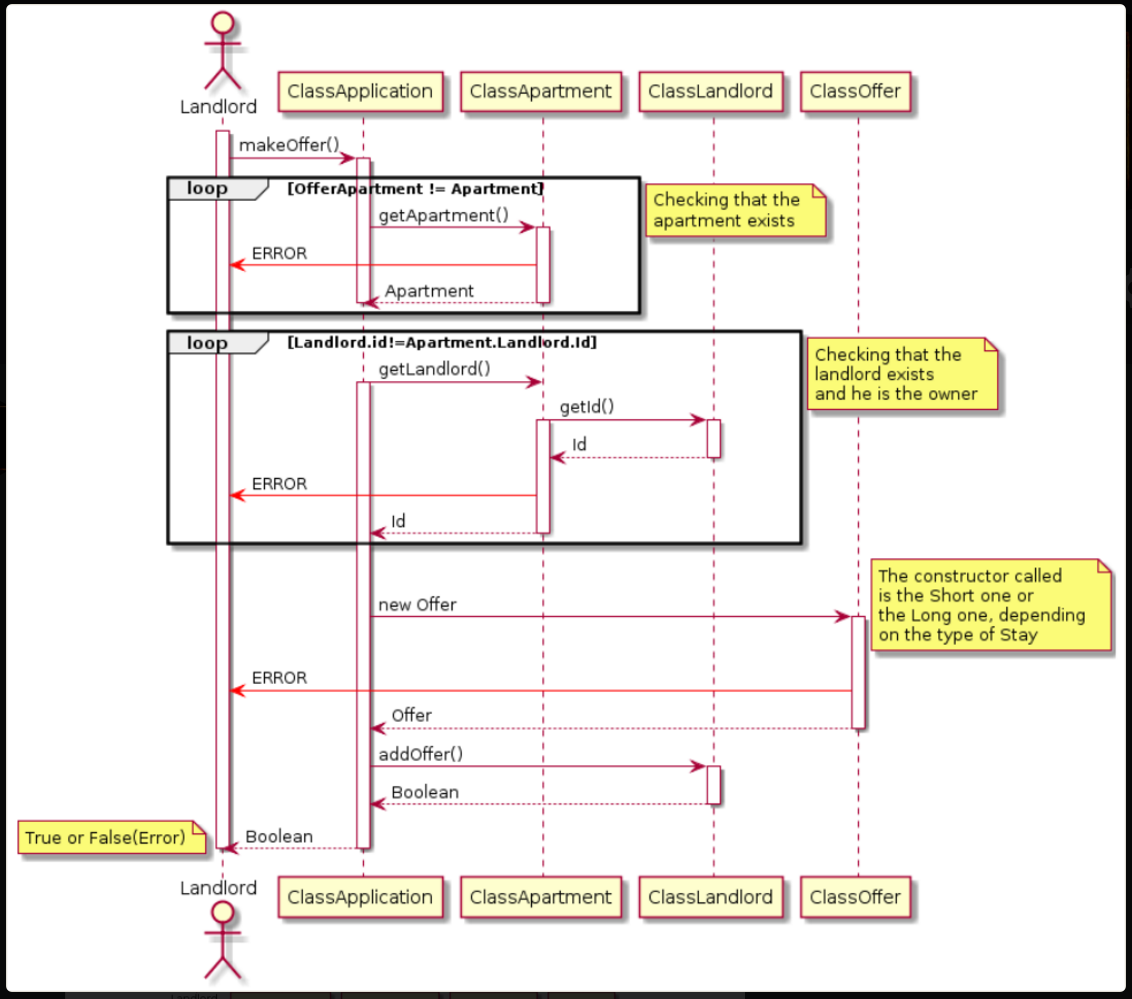
\includegraphics[scale=1]{sequence2.PNG}
\end{center}
The sequence that making a offer follows is not simple, but not very complicated either. First, the system checks if the offered property is already registered, then it makes sure the owner of the accommodation is the same than the landlord making the offer. Finally, if everything went OK, it calls the constructor of Short or Long offers (depeding on its type) and it adds the new offer to the register of all offers in the class application.

\subsection{Register and apartment sequence diagram}
Here we are presenting the sequence diagram of registering a property. It is simpler that the previous one.
\begin{center}
	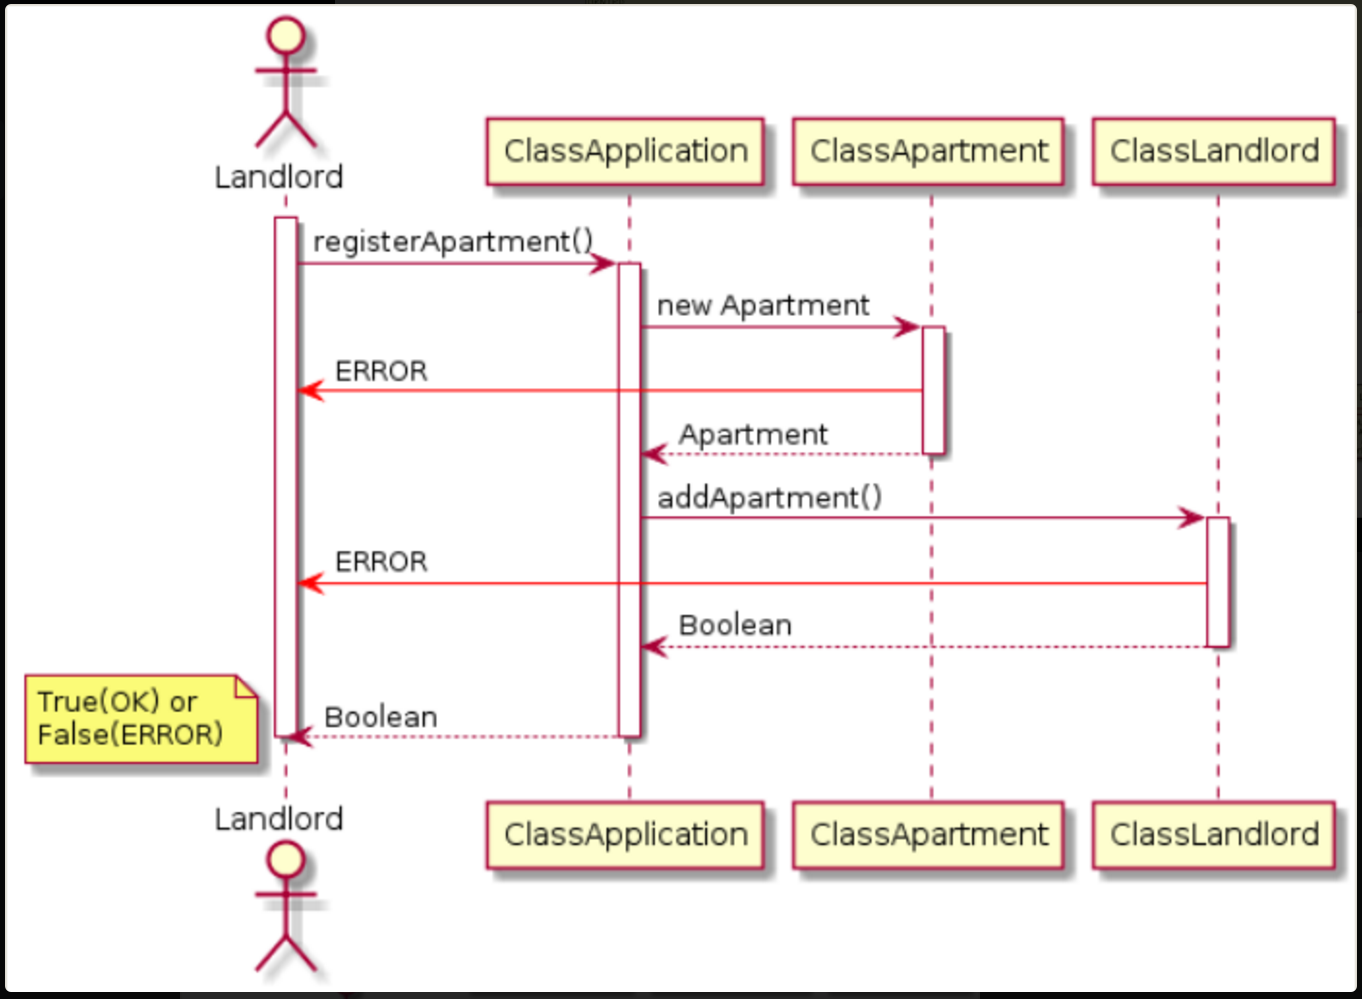
\includegraphics[scale=1]{sequence1.PNG}
\end{center}
It just creates a new apartment with its constructor, then it adds it to the register of all apartment that the landlord has, and finally, it puts the new apartment in the register of all properties of the application. It is the main scenario, but remember that error might occur, so in the diagram are shown those possibilites as well.

\section{Requirements traceability matrix}
To end, we are attaching to this document several traceability matrixes due to its huge size if we put all together.\\\\
In the Y-axis there are written the different requirements, and in the X-axis, appear the different methods that works in order to satisfy theese requirements.\\\\
It important to keep in mind that Registered User requirements includes Non-Registered User requirements, and so its methods. For the same reason, Landlord-Renter matrix is a combination of Renter matrix plus Landlord matrix.\\\\
The only matrix that has no influence on others, is the Manager traceability matrix, because it just has to gather the manager requirements.

\section{Conclusion}
It has been a difficult practice because of the fact it was our first time designing a project, at the same time that we are learning Java, but we think we have managed to overcome it, and we are looking forward to improve in the next design diagrams.

\end{document}